\label{Test_Kapitel}
\section{Test}
In den Tests ging es darum, die in Kapitel 4 gezeigten Lösungen zu validieren.
Das Ziel dieser Tests ist es in erster Linie, die gesetzten Anforderungen auf ihre Erfüllung zu testen. Des Weiteren sollen die Tests vorbeugen, dass Änderungen während der fortlaufenden Entwicklung unbemerkt zu einem Versagen der Erweiterung führen. Um das Ziel möglichst effizient zu erreichen, bedarf es einer Teststrategie. Diese soll hier Vorgestellt und die Umsetzung erläutert werden. Darüber hinaus sollen weitere Testmöglichkeiten erörtert werden.
\subsection{Teststrategie}
%, die dann bereits getestete Schnittstelle und damit verbundenen Abläufe Fehler integriert werden. Vor allem funktionale Tests benötigt werden. Da aufgrund der Architektur der Erweiterung viele unabhängige Module miteinander interagieren, sollten hierfür alle Testebenen abgedeckt werden. Dabei sollen sowohl manuelle Tests zum Einsatz kommen als auch bereits vorgestellte Tools wie z. B. QTest und der kontinuierlichen Integration. Hierfür wurden die folgenden Teststrategien erstellt:
%\begin{enumerate}
%	\item Zur Überprüfung der Anforderungen sollen funktionale Systemtests entworfen werden. Diese sollen auf der Basis typischer Nutzeraktionen erstellt werden und deshalb auch manuell durchgeführt werden. Diese werden in einer Tabelle als ein Testprotokoll festgehalten.
%	\item Integrationstests: Hiermit sollen einzelne Abläufe im Code abgedeckt werden. Diese sollten mithilfe des QTest Frameworks erstellt werden und automatisch ablaufen. Hier bietet es sich auch an über mehrere
%	\item 
%\end{enumerate}Um die Konsistenz innerhalb des Projektes zu bewahren und den Aufwand geringer zu halten, bietet es sich an auf bereits bestehenden Tests aufzubauen.
Es sind bereits Tests im Projekt Tankautomat vorhanden. Diese bauen auf dem Regressionstest Prinzip auf (vgl. \cite{Ba_Miriam}, S.18). Dieses Prinzip beschreibt das erneute Testen der Applikation nach einer Änderung unter der Verwendung bereits erstellter Tests (vgl. \cite{Basis_Tests}, S.98). Dabei werden sowohl Funktionale als auch Nicht-Funktionale Aspekte der Software getestet. Dies bedeutet, dass alle (Teil-) Systeme z. B. Klassen oder Funktionen darauf geprüft werden, ob sie ihre Aufgabe erfüllen (Funktional) und mit welcher Qualität/Performance diese Aufgaben erfüllt werden (Nicht-Funktional)(vgl.\cite{Basis_Tests}, S.87 \& S.89). Diese Aspekte werden auf unterschiedlichen Testebenen getestet. Die Testebenen sind analog zu einem Softwaresystem aufgeteilt. Wobei Tests für abgekapselte Systeme, z. B. Klassen als sog. \textit{Unittests} oder Komponententests bezeichnet werden. Integrationstest überprüfen die Interaktion dieser \textit{Units} und stehen somit eine Ebene über den Unittests. Als höchste Testebene werden die sog. Systemtest angesehen, da diese aus vielen dieser Interaktionen bestehen (vgl.\cite{Basis_Tests}, S.62ff.). Bis auf die Systemtests werden alle Tests im Projekt über die kontinuierliche Integration, automatisch nach einer Codeänderung ausgeführt. Die Systemtests werden manuell an einem Prototypenaufbau, mit der Hilfe eines Testprotokolles durchgeführt. Um die Konsistenz im Projekt beizubehalten, macht es also Sinn sich an diesem Vorgehen zu orientieren und eines dieser Testprinzipien zu übernehmen. Die Wahl soll hier begründet und die Umsetzung erläutert werden.
\subsubsection{Validierung der Anforderungen}
%Irgendwie noch auf OCPP2.0.1 eingehen
Da die Anforderungen an die Erweiterung sehr allgemein gehalten wurden und mehr aus der Nutzerperspektive beschrieben sind, bot es sich an, die Tests auf der Systemebene durchzuführen. Dabei konnte die bereits bestehende Testart für Systemtests adaptiert werden, um die Anforderungen zu validieren. Der Nachteil dieser Tests ist allerdings, dass sie aktiv von einer Person durchgeführt und dokumentiert werden müssen. In diesem Anwendungsfall gab es aber vor allem drei ausschlaggebende Vorteile:
\begin{enumerate}
	\item Die Tests können bereits während der Entwicklung eingesetzt werden.
	\item Sie sind ohne viel Zeit und Aufwand erstellbar.
	\item Sie können direkt auf der Hardware eingesetzt werden.
\end{enumerate}
Aus diesem Gründen wurde sich für eine manuelle Testmethode entschieden.
\subsubsection{Testplanung}
Um die Erweiterung komplett zu testen, müssen alle Anforderungen abgedeckt werden. Hierfür soll eine Testspezifikation entworfen werden, die den Tester durch alle Szenarien, die in den Anforderungen beschrieben sind, leiten. Dabei sollen immer eine Konfiguration, Eingabe und ein erwartetes Ergebnis vorgegeben werden. Der Tester dokumentiert anhand des Vergleiches von erwartetem und tatsächlichen Ergebnis, ob der Test erfolgreich war oder nicht. Bei einem unerfolgreichem Testergebnis, sollten zusätzliche Informationen angegeben werden. Die Voraussetzung beschreibt die Konfiguration des Tankautomaten, für die der Test durchgeführt werden soll. Die Eingabe nennt die Schritte, um den Test durchzuführen. Alle vom Protokoll abhängigen Tests, z. B. Starten eines Ladevorgangs, sollten für beide Protokollversionen durchgeführt werden.
\subsubsection{Testumgebung} \label{Testumgebung}
Die manuellen Tests sollten an einem Testaufbau erfolgen. Um beide Versionen des Protokolls testen zu können, sollten die Tests für jeweils mindestens eine Ladesäule, die mit OCPP1.6 konfiguriert ist und für eine, die mit OCPP2.0.1 konfiguriert ist, durchgeführt werden. Hierfür muss die im System angeschlossene Ladesäule, beide OCPP Versionen unterstützen oder es müssen zwei getrennte Ladesäulen verwendet werden. Für eine bessere Vergleichbarkeit der beiden Protokollversionen sollte ersteres bevorzugt werden.\newline
\noindent Als Alternative zum Testaufbau kann die Applikation ebenfalls mit einer \acfi{VM} simuliert werden, in dem der Desktop Build genutzt wird. Die Ladesäule kann mithilfe eines OCPP Simulators nachgestellt werden. Für OCPP1.6 bietet sich der bereits erwähnte MicroOcppSimulator an. Für OCPP2.0.1 ist leider keine vergleichbare Alternative vorhanden. Hier müsste z. B., mit der ebenfalls erwähnten Python Bibliothek \glqq{}Mobilityhouse-ocpp\grqq{} eine vergleichbare Applikation erstellt werden.
\subsection{Umsetzung}
Für die Erstellung der manuellen Tests wurde sich an den typischen Tankabläufen orientiert. Die anbei gezeigten Testspezifikationen enthalten immer die Anforderung, die durch den Test abgedeckt wird. Es wurden immer mehrere Testfälle gewählt, um eine Anforderung abzudecken. Je nach Formulierung der Anforderung konnten mehrere Testfälle für diese entworfen werden. Es wurde darauf geachtet, das mindestens immer eine negative und positive Überprüfung in den Tests enthalten ist. Damit ist ausgeschlossen, dass die Anforderung nur zufällig erfüllt ist. Als Beispiel kann hierfür die Testspezifikation für die Anforderung T-02 betrachtet werden. Diese ist in \autoref{fig:Testspezifkationen_man} zu sehen.\newline
\begin{figure}[H]
	\centering
	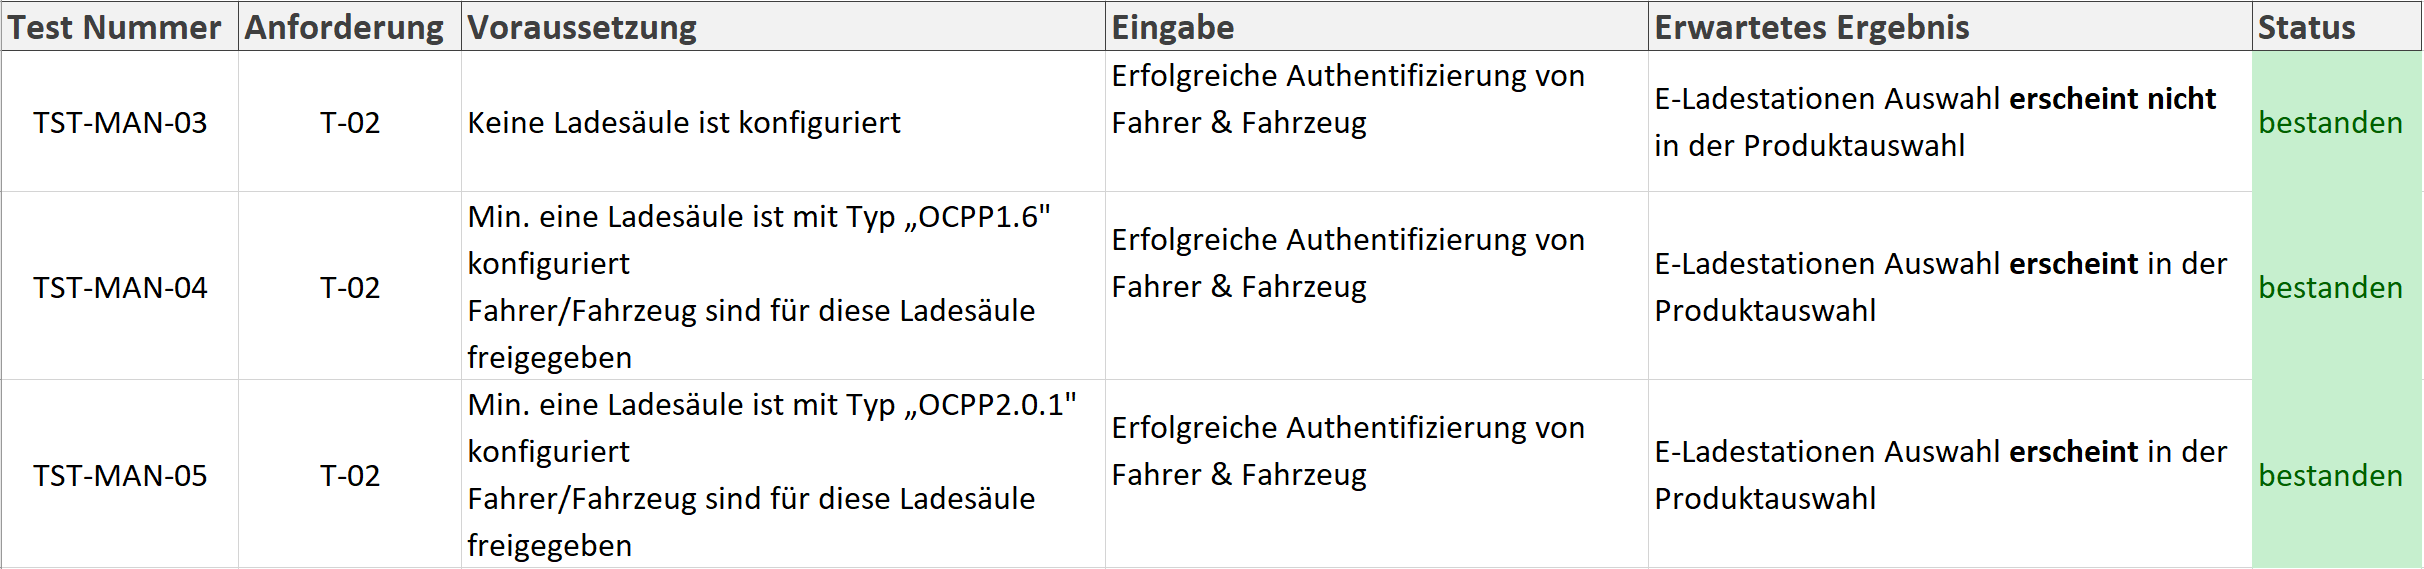
\includegraphics[width=1.0\textwidth]{images/Test/Ausschnitt_manuelle_TestSpezifikationen.png}
	\caption{Ausschnitt der manuellen Testspezifikationen \cite{Eigene_Darstellung}}
	\label{fig:Testspezifkationen_man}
\end{figure}
\noindent Hier sind die positiven Testergebnisse in TST-MAN-04 und TST-MAN-05 beschrieben und entsprechen der in der Anforderung genannten Spezifikation. TST-MAN-03 prüft den gegenteiligen Fall ab, der nur implizit in der Anforderung genannt wurde. Diese Testspezifikationen wurden für alle aufgezählten Anforderung erstellt und sind in \autoref{Anhang:man_test} zu finden.

\subsubsection{Durchführung}
Die manuellen Tests wurden anfangs mithilfe des MicroOcppSimulators und fortschreitend mit zwei Ladesäulen des Kunden getestet. Dabei handelte es sich zum einen um eine Ladesäule des Herstellers \glqq{}Alfen\grqq{} und um eine des Herstellers \glqq{}Wallbe\grqq{}. Die Alfen Ladesäule unterstützte beide Protokollversionen und wurde jeweils für eine Protokollversion in den Tests konfiguriert. Die Wallbe Ladesäule unterstützte nur die Version 1.6 des Protokolls. Beide wurden über einen \textit{Unmanaged Switch} mit dem Terminal verbunden und für die Tests entsprechend in der Cloud Weboberfläche konfiguriert. Um das Anschließen der Fahrzeuge zu simulieren, kamen hierfür spezielle Testgeräte zum Einsatz, an denen über Drehknöpfe der Zustand des Fahrzeuges simuliert werden konnte. Zusätzlich konnte auch über eine Steckdose, ein einphasiger Wechselstrom Verbraucher angeschlossen werden, um einen Ladevorgang zu simulieren. 
Der Simulator wurde zusätzlich eingesetzt, um schnelle Tests ohne den Testaufbau durchzuführen oder um ein schwerwiegendes Problem zu debuggen. Hierfür wurde die Desktopversion der Tankautomaten Applikation genutzt. Die finalen Ergebnisse wurden wie beschrieben in der Testspezifikation festgehalten. 
\subsubsection{Ergebnisse}\label{Testergebnisse}
Es konnten alle Testszenarien durchgegangen werden, mit der Ausnahme von den Tests für die Anforderung C-01. Die Testergebnisse konnten aufgrund der fehlenden Integration auf Cloud Seite nicht verifiziert werden. Dabei konnten mit dem MicroocppSimulator und mit der Alfen Ladesäule, alle Anforderungen verifiziert werden. Bei der Wallbe Ladesäule kam es allerdings zu Problemen, da diese Abweichungen in der Protokollimplementierung hatte. So wurde vom Hersteller der Ladesteuerung zwar angegeben, dass der Parameter \spverb|MeterValuesSampledData| alle Messwerte beinhaltet (\cite{Wallbe_Steuerung}, S.42ff.), aber bei der Abfrage des Parameters wurde ein ungültiger Wert: \glqq{}true\grqq{} zurückgegeben. Dieser ist laut OCPP Doku nicht für diesen Konfigurationsparameter erlaubt (vgl.\cite{OCPP-1.6-edition-2}, S.86ff.). Außerdem konnte beobachtet werden, dass eine Transaktion über den Befehl \spverb|StartTransaction| gestartet wird, allerdings werden danach keine \spverb|MeterValues| Nachrichten versendet und die Transaktion nicht über \spverb|StopTransaction| beendet. Damit war es nicht möglich Transaktion zu beenden, oder währenddessen die Lademenge zu erfahren. Zum Zeitpunkt dieser Arbeit konnte bisher kein Grund für dieses Verhalten gefunden werden. Da aber bereits durch den ungültigen Wert gegen das Protokoll verstoßen wurde und dieses Verhalten weder bei der Alfen Ladesäule noch beim MicroocppSimulator beobachtet wurde, kann davon ausgegangen werden, dass sich die Ladesäule auch in diesem Fall nicht an das OCPP Protokoll hält. Hier muss zukünftig durch weitere Tests (siehe \autoref{Testeröterung}) festgestellt werden, ob es sich um einen Fehler bei der Ladesäule oder beim Tankautomaten handelt.\\

\noindent Neben diesem konnten, auch während der Entwicklung bereits wichtige Fehler frühzeitig erkannt und behoben werden (siehe \autoref{OCPP Probleme Umsetzung}). Da die durchgeführten Tests allerdings nur sehr allgemein gehalten wurden, sollten für spezifischere Tests, vor allem mit Blick auf die OCPP Schnittstelle, andere Testarten miteinbezogen werden. Des Weiteren ist die andauernde Durchführung von manuellen Tests sehr Zeit intensiv und dementsprechend unwirtschaftlich, da diese Zeit auch die Entwicklung oder Verbesserung von Testergebnissen gesteckt werden könnte. Deshalb wurden auf Basis dieser Erkenntnisse, weitere Testmöglichkeiten erörtert, aber nicht umgesetzt. 
\subsection{Erörterung weiterer Testmöglichkeiten}\label{Testeröterung}
Die Anforderungen wurden zwar erfolgreich durch die manuellen Tests an einer Ladesäule und dem Simulator abgedeckt werden, allerdings wurden durch diese Tests viele Testaspekte offengelassen. Um ein weiteres Vorgehen zu planen, sollen in Folge der Erkenntnisse aus den Testergebnissen einige weitere Testmöglichkeiten, als Empfehlung für das Entwicklerteam und das Unternehmen ausgesprochen werden.
\subsubsection{Nicht-funktionale Tests}
Die jetzigen Tests beinhalten nur die Überprüfung der Anforderung und prüfen somit nur funktional. Da der Tankautomat später in Szenarien eingesetzt wird, in dem viele Ladesäulen über diesen verwaltet werden müssen, sollten ebenfalls nicht-funktionale Tests eingeführt werden. Diese sollten die Performance der Erweiterung testen, in dem sich viele Ladesäulen verbinden und gleichzeitig Nachrichten senden. Hierfür würde sich erneut die Mobilityhouse OCPP Bibliothek anbieten, mit der ein Python Skript erstellt werden kann, um mehrere Ladesäulen zu simulieren. Dieses Skript kann für manuelle Tests an der Hardware genutzt werden. Es sollte aber besser umsetzbar als automatischer Test sein, da hier leichter mehrere Ladesäulen Instanzen erstellt werden können und diese auch in die kontinuierliche Integration mit einbezogen werden können.
\subsubsection{Komponententests}
Um die einzelnen hinzugefügten Klassen und darin enthaltene Funktionen zu testen, können Komponententests hinzugefügt werden. Diese können über das Qt Test Framework realisiert werden. Dieses Vorgehen kann vor allem für die Überprüfung der einzelnen OCPP Nachrichten gut realisiert werden, in dem z. B. Variablen für ein Nachrichtenobjekt gesetzt werden. Über die \verb|createConfirm| oder \verb|createRequest| Methode kann dann ein JSON Payload generiert werden. Dieser kann dann mit dem erwarteten JSON Payload über \verb|QCompare| verglichen werden.
\subsubsection{Integrationstests}
Als Ergänzung zu den Komponententests können ebenfalls Integrationstests sinnvoll sein. Diese können dasselbe Prinzip der Komponententests übernehmen, aber dafür ganze Nachrichtenverläufe abfragen oder z. B. den Transaktionsstart simulieren. Um dies zu erreichen, kann wieder über Qt Test eine vollständige OCPP Nachricht vorgegeben werden und erneut mit einer erwarteten Antwort vergleichen werden. So können auch besser Sonder-, Grenz- und Extremfälle getestet werden. Wie z. B. die Fehler auf eine nicht korrekt formatierte Nachricht oder Probleme beim Übertragen der Nachricht. Mit diesen Tests kann auch leichter das unerklärte Verhalten der Wallbe Ladesäule nachgestellt und weiter erforscht werden. 
\newpage
